\chapter{Conclusões}
\label{cap:conclusoes}

O Capítulo~\ref{cap:avaliacao} mediu cada componente isoladamente. Este reúne o que dessas
medições se retira. Sintetiza o trabalho realizado, apresenta a resposta obtida para cada questão de
investigação, identifica as limitações do estudo e enuncia as linhas de desenvolvimento futuro.

\section{Conclusões principais}
\label{sec:con_principais}

O trabalho produziu um sistema em funcionamento e uma avaliação de cada uma das técnicas que o
compõem. O InvestiGator monitoriza doze empresas em ciclo contínuo, entrega alertas explicados a um
canal público e disponibiliza uma página onde ficam registadas tanto as mensagens enviadas como as
decisões que conduziram ao silêncio. Ao longo do período documentado no
Capítulo~\ref{cap:avaliacao} foram entregues $367$ mensagens e registadas $4\,366$ decisões de
triagem, e a base de precedentes acumulou $38\,214$ casos com impacto medido. Estes números
descrevem um sistema implantado e não uma demonstração construída para o efeito.

A componente que confere ao trabalho o carácter de dissertação não é, contudo, o sistema, mas a
avaliação a que foi submetido. Três das quatro técnicas foram comparadas com alternativas mais
simples, escolhidas e declaradas antes de a medição ser realizada, o que é a condição para que o
resultado possa ser negativo. Numa delas o resultado foi efetivamente negativo. A quarta técnica, a decomposição do movimento, não admite comparação da mesma natureza, uma vez
que a repartição de um retorno não possui referente externo observável. Dela mediu-se o que
permanece falsificável: a qualidade do ajuste que a sustenta, e a capacidade de produzir respostas
distintas para empresas distintas.

A contribuição de engenharia não reside na dimensão do modelo aprendido. O sistema treina um único
modelo, com nove entradas, e esse modelo perde para uma linha de base de uma só variável. A confiança nesse valor, e na conclusão negativa que ele sustenta, depende do que foi preciso
construir em volta dele. A Secção~\ref{sec:sis_ciclo} descreve as seis peças. O conjunto de dados
é rotulado a partir de duas fontes independentes. A separação temporal é verificada por um
procedimento automático. A calibração vem acompanhada da medição e da declaração do enviesamento
que a afeta. Os artefactos ficam sob controlo de versões. O modelo implantado é comprovadamente o
modelo avaliado. E o sistema em funcionamento continua a ser observado. É nesse conjunto, e não no
modelo, que reside o trabalho.

Uma segunda conclusão atravessa os quatro casos de estudo e não pertence a nenhum deles em
particular. Em três ocasiões distintas, uma técnica mais simples obteve melhor resultado do que uma
técnica mais sofisticada em condições equivalentes: o \emph{z}-score deslizante contra dois
detetores aprendidos, a volatilidade recente contra as representações de texto, e uma tabela de
treze constantes contra o modelo treinado. Em três outras ocasiões sucedeu o inverso, com a alternativa medida a obter melhor resultado. O
sistema conservou a opção implantada por razões distintas em cada caso: o estimador de pesos
iguais por explicabilidade, a janela de vinte dias por responsividade, e o codificador de frases
mais pequeno por custo computacional.

A distinção entre estes dois casos é a distinção entre resultado e escolha, e o
presente capítulo mantém-na explícita: o que a medição estabelece é reportado como resultado, e o
que o autor decidiu apesar da medição é reportado como decisão, acompanhada do que essa decisão
custa quando a medição separa as alternativas, e da declaração de que nada custa em \gls{PRAUC}
quando não as separa.

\section{As respostas às questões de investigação}
\label{sec:con_respostas}

Esta secção responde às três questões enunciadas na Secção~\ref{sec:intro_objetivos} e delimita, em
cada caso, o que a resposta permite e não permite afirmar. A Figura~\ref{fig:con_scorecard} reúne as
três.

\begin{figure}[ht]
\centering
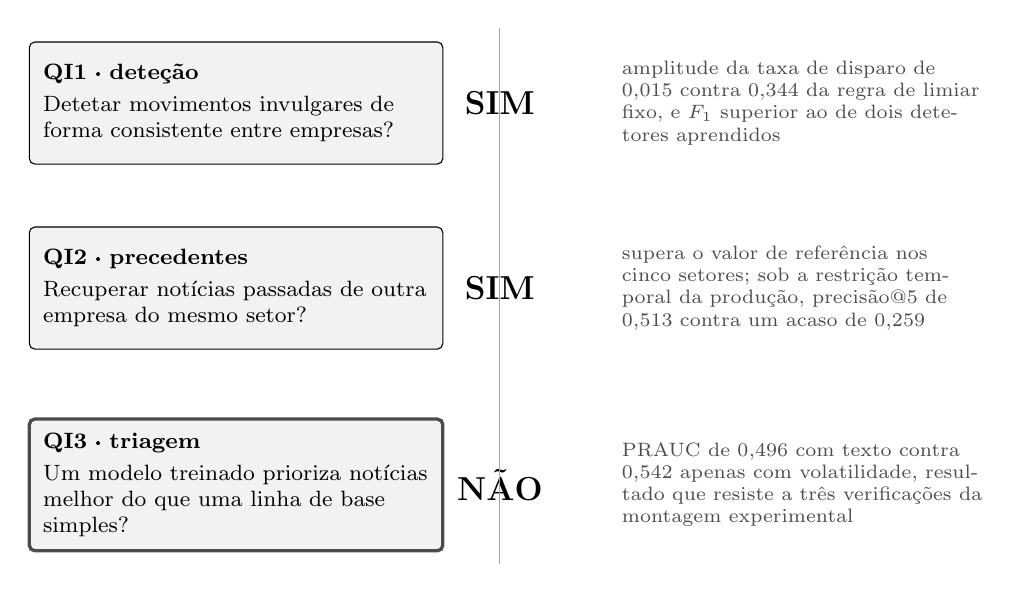
\begin{tikzpicture}[font=\footnotesize,
  cx/.style={draw, rounded corners=2pt, align=left, inner sep=5pt, text width=4.9cm,
             minimum height=1.55cm, fill=black!5},
  neg/.style={cx, draw=black!70, very thick},
  ver/.style={font=\bfseries\large, align=center},
  num/.style={align=left, text width=4.6cm, font=\scriptsize, text=black!70},
]
  \node[cx] (q1) at (0,0) {\textbf{\gls{QI}1 · deteção}\\[2pt]
    Detetar movimentos invulgares de forma consistente entre empresas?};
  \node[ver] at (3.35,0) {SIM};
  \node[num] at (7.2,0) {amplitude da taxa de disparo de $0{,}015$ contra $0{,}344$ da regra de
    limiar fixo, e $F_1$ superior ao de dois detetores aprendidos};

  \node[cx] (q2) at (0,-2.35) {\textbf{\gls{QI}2 · precedentes}\\[2pt]
    Recuperar notícias passadas de outra empresa do mesmo setor?};
  \node[ver] at (3.35,-2.35) {SIM};
  \node[num] at (7.2,-2.35) {supera o valor de referência nos cinco setores; sob a restrição
    temporal da produção, precisão@5 de $0{,}513$ contra um acaso de $0{,}259$};

  \node[neg] (q3) at (0,-4.85) {\textbf{\gls{QI}3 · triagem}\\[2pt]
    Um modelo treinado prioriza notícias melhor do que uma linha de base simples?};
  \node[ver] at (3.35,-4.85) {NÃO};
  \node[num] at (7.2,-4.85) {\gls{PRAUC} de $0{,}496$ com texto contra $0{,}542$ apenas com
    volatilidade, resultado que resiste a três verificações da montagem experimental};

  \draw[black!35] (3.35,-5.85) -- (3.35,0.95);
\end{tikzpicture}
\caption[As três questões de investigação e as respostas obtidas]{As três respostas, com a resposta
negativa apresentada com o mesmo destaque das duas restantes. A terceira linha é a que atribui
crédito às outras: um trabalho que reporte apenas os resultados favoráveis não permite determinar se
as respostas afirmativas foram medidas ou pressupostas.}
\label{fig:con_scorecard}
\end{figure}

\subsection{Deteção de movimentos invulgares}

A resposta à \gls{QI}1 é afirmativa. Um \emph{z}-score sobre uma janela deslizante de vinte dias assinala dias raros a uma taxa
praticamente idêntica em empresas de volatilidades muito distintas. A amplitude entre a empresa
mais e a menos assinalada é de $0{,}015$, contra $0{,}344$ de uma regra de limiar fixo em três por
cento. Contra um rótulo aproximado, o método obtém
$F_1 = 0{,}516$ e a regra fixa $0{,}218$. Sujeito a um protocolo causal equivalente, o mesmo método
supera ainda dois detetores concebidos para esta tarefa, com $F_1$ de $0{,}530$ contra $0{,}269$ do
\emph{Isolation Forest} \autocite{liu2008isolation} e $0{,}280$ do \emph{Local Outlier Factor}
\autocite{breunig2000lof}.

A configuração implantada não é, porém, a melhor medida dentro da própria família. Com a mesma
cobertura, um estimador com decaimento exponencial obtém $F_1 = 0{,}664$ e uma janela de sessenta
dias obtém $0{,}678$, contra os $0{,}516$ da configuração em produção. O que a \gls{QI}1 estabelece
é que a família deslizante supera o limiar fixo e os dois detetores aprendidos, e não que a
parametrização escolhida seja a melhor dessa família.

Este resultado é menos surpreendente do que a diferença de valores sugere, e a literatura permite
situá-lo. Os dois detetores aprendidos definem raridade a partir da geometria dos dados, um por
isolamento do ponto e outro por comparação de densidades, e foram concebidos para espaços com
múltiplas variáveis em interação. O problema tratado apresenta uma única série de retornos por empresa, na qual a estrutura
relevante é temporal e não geométrica: períodos de agitação sucedem-se a períodos calmos. É a
propriedade que os modelos \gls{ARCH} e \gls{GARCH} formalizam \autocite{engle1982arch,
bollerslev1986garch}. A janela deslizante capta-a diretamente; um detetor treinado sobre o
conjunto completo teria de a aprender. Quando a suposição embutida
num método simples coincide com a estrutura efetiva do problema, a margem para a superar é reduzida.

O alcance da resposta é delimitado por três condições. A comparação incide sobre quinze empresas de
grande capitalização, selecionadas em 2026 e avaliadas sobre o passado, que sobreviveram por
construção; sobre três anos de cotações e sobre um único mercado. O rótulo utilizado como argumento
secundário é ele próprio relativo à volatilidade de cada empresa, razão pela qual o argumento
principal é a consistência da taxa de disparo, que não depende de rótulos. O limiar de três por cento
da regra alternativa não foi otimizado, pelo que o que a comparação estabelece não é que nenhum
limiar fixo obtivesse melhor resultado, mas que uma regra de limiar fixo mede uma quantidade distinta
da pretendida.

\subsection{Recuperação de precedentes}

A resposta à \gls{QI}2 é afirmativa, e a sua formulação exige o nível do setor. Sobre o corpus
recente, a recuperação por semelhança de frase \autocite{reimers2019sbert} obtém precisão@5 de
$0{,}514$, contra $0{,}346$ da sobreposição de vocabulário, $0{,}240$ da escolha aleatória e
$0{,}126$ da apresentação das notícias mais recentes. Também aqui o modelo implantado não é o melhor
medido: uma variante de maior dimensão obtém $0{,}538$ sobre o mesmo protocolo, e foi preterida por
custo computacional.

O valor agregado não constitui, porém, a forma adequada de enunciar o resultado. Quase metade das
notícias do corpus pertence ao setor da tecnologia, o que torna disponível uma estratégia que
dispensa qualquer modelo e sequer observa a consulta, consistindo em devolver invariavelmente
notícias desse setor; a sua precisão iguala a fração de consultas de tecnologia, $0{,}467$. Essa
estratégia é inútil enquanto produto, dado que acerta em todas as consultas de um setor e em nenhuma
dos quatro restantes, mas a sua existência demonstra que o agregado mede em parte a composição do
corpus.

A comparação que resiste à objeção realiza-se dentro de cada setor, onde o método supera o
respetivo valor de referência nos cinco. A margem absoluta é maior no setor mais abundante, com
$+0{,}283$ na tecnologia; nos setores escassos, onde o valor de referência ronda $0{,}072$, o método
obtém várias vezes esse valor com margem absoluta menor. É esta a afirmação que o trabalho
sustenta.

Duas verificações adicionais delimitam a resposta. Sobre o corpus histórico completo, com aproximadamente oitenta mil notícias de seis anos, a
precisão sobe para $0{,}595$. O valor de referência sobe na mesma proporção, e a margem mantém-se.
O método não se degrada com a escala, nem melhora com ela. A imposição da restrição que o sistema
efetivamente enfrenta, segundo a qual o precedente tem de ser anterior à consulta, reduz a precisão
para $0{,}513$ e o valor de referência para $0{,}259$, com a margem a variar $0{,}008$. O método
conserva a vantagem quando obrigado a operar como opera em produção.

A segunda ressalva tem consequências diretas sobre o produto. A recuperação identifica tema e não
direção: a concordância entre o sentido do movimento da notícia de consulta e o dos precedentes
situa-se em $0{,}708$ contra um valor de acaso de $0{,}688$, uma diferença de $0{,}020$. Duas
notícias podem tratar do mesmo assunto e o preço evoluir em sentidos opostos. O resultado é
coerente com o que a forma semiforte da hipótese dos mercados eficientes conduziria a esperar
\autocite{fama1970efficient}, segundo a qual a informação pública se encontra já refletida no preço,
sem que o trabalho a teste ou nela se apoie para estabelecer qualquer conclusão. A consequência
prática é a decisão de apresentar os precedentes individualmente, com data e desfecho, em vez de os
resumir a uma média suscetível de ser lida como previsão.

Uma delimitação final respeita ao rótulo. A pertença ao mesmo setor é uma aproximação verificável de
relevância, e não a propriedade que se pretendia medir. A linha de base lexical é a forma mais elementar da sua família, sem ponderação pela raridade dos
termos nem normalização pelo comprimento. Os dezassete pontos percentuais de vantagem medem a
distância a um ponto de partida, e não a uma função de ordenação afinada
\autocite{robertson2009bm25}.

\subsection{Triagem de notícias}

A resposta à \gls{QI}3 é negativa. Nenhuma variante que incorpora o texto do título supera uma linha
de base construída apenas com a volatilidade dos vinte dias anteriores, com $0{,}496$ de \gls{PRAUC}
contra $0{,}542$, e o índice de Brier acompanha a mesma ordenação. O resultado resiste a três verificações. A primeira repete a comparação concedendo ao texto as
melhores condições disponíveis, e eleva o seu melhor valor para $0{,}533$, sem alcançar a linha de
base. A segunda reamostra por grupos constituídos pela empresa e pelo dia, e mantém o intervalo a
excluir zero. A terceira repete a medição para nove combinações alternativas de limiar e horizonte
do rótulo, e a volatilidade iguala ou supera o modelo com texto nas nove.

A resposta ganhou precisão no decurso do trabalho e essa precisão altera o que dela se retira. As
comparações anteriores colocam as representações lado a lado e respondem, por conseguinte, à pergunta
sobre qual delas é melhor. A pergunta com maior utilidade para quem constrói um sistema é distinta e
consiste em determinar se o texto acrescenta ao que já é conhecido. Medida sobre a tabela de consulta
por empresa, que contém tudo o que o modelo conhece da empresa e nada da notícia, a resposta é
afirmativa: o título acrescenta $+0{,}012$ de \gls{PRAUC}, com intervalo entre $+0{,}004$ e
$+0{,}020$, que exclui zero. É a única ocasião em que uma representação de texto apresenta um
acréscimo detetável nesta tarefa.

O valor situa-se abaixo do limite de $0{,}02$ que o Capítulo~\ref{cap:avaliacao} fixou antes das
medições, e esse limite aplica-se nos dois sentidos. Fica estabelecido um limite superior para o
efeito do texto, e não uma quantidade de que o sistema possa dispor.

Três medições impedem que este acréscimo reabra o veredicto. A soma não supera a volatilidade isolada, e o intervalo da diferença contém zero. O acréscimo não
sobrevive à métrica que descreve o produto: a precisão dentro do orçamento de cinco alertas por
dia permanece em $0{,}662$ com e sem texto. E a capacidade de separar notícias da mesma empresa
mantém-se ao nível do acaso. O que estas medições acrescentam à resposta negativa não é uma ressalva mas uma localização: a
informação que o texto transporta distingue empresas e períodos, quando o produto necessitava de
distinguir notícias. A formulação que subsiste é a mais fraca das possíveis, correspondendo a um
limite superior de um efeito e não a uma descoberta.

Existe uma linha de investigação estabelecida que utiliza texto para antecipar movimentos de preço
\autocite{xing2018nlffsurvey, ding2015deep}, e este resultado não a contradiz. A diferença não reside na dimensão do texto, uma vez que \textcite{ding2015deep} operam igualmente
sobre títulos, mas no tratamento que lhe é dado. Aqueles autores extraem estruturas de
acontecimento e treinam uma rede para prever a direção do movimento. Aqui os títulos são
comparados por semelhança, e a direção nunca é objeto de previsão. Os corpora e os horizontes de avaliação diferem igualmente. A
afirmação que este trabalho sustenta é mais estreita do que uma refutação: sob esta restrição de
dados e com esta família de métodos, o sinal textual nada acrescenta ao que a volatilidade recente
já indicava. O alcance do resultado limita-se, por isso, a um regime de recursos e a uma escolha de
representação, e não se estende à linguagem.

Há, ainda assim, uma leitura teórica que o enquadra e que convém enunciar com a mesma cautela. A
forma semiforte da hipótese dos mercados eficientes \autocite{fama1970efficient} sustenta que a
informação publicamente disponível se encontra já refletida no preço. Se assim for, um título
público não tem, no momento em que é lido, informação que os preços recentes não contenham, e o
resultado obtido é o que essa hipótese conduziria a esperar. A condição de recursos deste trabalho
agrava a expectativa em vez de a atenuar: entre a publicação de uma notícia e a sua deteção por
fontes gratuitas decorrem $353$ minutos de mediana, intervalo durante o qual qualquer reação do
mercado já ocorreu. O sistema observa, por construção, informação que deixou de ser nova.

Esta leitura é um enquadramento e não uma conclusão. O trabalho não testa a hipótese dos mercados
eficientes, e um resultado negativo obtido com uma família de métodos sobre um corpus concreto não
a confirma; confirmá-la exigiria um desenho que este não tem. O que a leitura acrescenta é a razão
pela qual o resultado é menos surpreendente do que a hipótese inicial supunha, e por que motivo a
sua correção mais provável não está na representação do texto mas no atraso com que ele chega.

\section{Objetivos alcançados}
\label{sec:con_objetivos}

Dos quatro objetivos enunciados na Secção~\ref{sec:intro_objetivos}, três encontram-se integralmente
cumpridos e um cumprido com a ressalva descrita adiante.

O primeiro objetivo, construir o sistema completo desde a aquisição de dados até à entrega do alerta,
está cumprido. Os dois gatilhos funcionam de ponta a ponta em produção, sobre fontes gratuitas, e o
percurso de um acontecimento está documentado no Capítulo~\ref{cap:sistema} com os valores de um caso
real.

O segundo objetivo, avaliar cada componente contra linhas de base transparentes, está cumprido
para as três técnicas em que existe um referente externo. Num dos casos foi além do previsto: o
detetor foi comparado não apenas com uma regra de limiar fixo, mas também com dois métodos
aprendidos.
A decomposição do movimento constitui a ressalva: não existe verdade de terreno contra a qual medir a
exatidão de uma repartição, pelo que se mediu o que nela permanece falsificável, correspondente à
qualidade do ajuste e à capacidade de discriminar. Ficaram por realizar comparações internas que
seriam possíveis, como a do modelo de um fator contra o de dois fatores ou a das sensibilidades
brutas contra as encolhidas.

O terceiro objetivo, garantir que as explicações apresentadas são fiéis ao que o sistema calculou,
está cumprido por construção e não por verificação posterior. Cada valor exibido provém do objeto que
o calculou, e o texto é composto a partir dessas peças, pelo que não é possível ao alerta enunciar um
valor distinto do que o sistema obteve. A fidelidade é, contudo, uma propriedade do sistema, e não da
relação entre o sistema e quem o lê; a utilidade das explicações para um investidor particular não
foi medida, e a Secção~\ref{sec:con_limitacoes} trata essa ausência.

O quarto objetivo, reportar os resultados obtidos incluindo os que não confirmem as expectativas
iniciais, está cumprido. A resposta negativa à \gls{QI}3 aparece na Figura~\ref{fig:con_scorecard}
e no corpo deste capítulo com o mesmo destaque das restantes, acompanhada das três verificações a
que foi submetida e das três ocasiões em que uma técnica mais simples superou uma mais
sofisticada.

\section{Limitações}
\label{sec:con_limitacoes}

Esta secção enumera as limitações do trabalho por ordem de importância. A
Tabela~\ref{tab:con_limites} apresenta-as em conjunto, com o trabalho que encerraria cada uma e a
natureza do respetivo custo; o texto que se segue desenvolve as quatro de maior consequência e
resume as restantes. A maioria está quantificada. Duas não o estão por natureza: a ausência de
avaliação com utilizadores é uma ausência e não uma medida, e a distância entre cada rótulo e a
propriedade que aproxima só seria mensurável contra uma anotação humana que não existe.

\begin{table}[!htbp]
\caption[As limitações e o trabalho que as encerraria]{As onze limitações, por ordem de
importância, com o trabalho que encerraria cada uma e a natureza do custo desse trabalho. As duas
que dependem de tempo de calendário são as que exigem julgamento humano, e são também as duas de
que as restantes mais dependem: enquanto não existir uma amostra anotada por pessoas, nem a
utilidade das explicações nem a qualidade dos rótulos deixam de ser aproximações.}
\label{tab:con_limites}
\centering
\footnotesize
\begin{tabular}{@{}L{0.33\textwidth} L{0.32\textwidth} L{0.20\textwidth}@{}}
\toprule
\tabhead{Limitação} & \tabhead{O que a encerra} & \tabhead{Custo} \\
\midrule
Nenhuma avaliação com pessoas & Executar o estudo desenhado, com seis a dez participantes &
tempo de calendário \\
A pontuação é quase constante dentro de cada empresa & Entradas que variem de um título para o
seguinte & reduzido \\
O rótulo pode favorecer a linha de base vencedora & Reconstruir o alvo com sensibilidades
estimadas & reduzido \\
Os rótulos são aproximações verificáveis & Anotar uma amostra com julgamento humano &
tempo de calendário \\
O alerta afirma mais evidência do que a que possui & Medir o impacto por notícia e não por dia &
dados intradiários \\
Os três blocos quase não partilham empresas & Uma divisão de composição constante & reduzido \\
Apenas o título é lido, e não o corpo do artigo & Recolher e representar o texto integral &
dados novos \\
A repartição nem sempre está bem estimada & Exibir o ajuste junto de cada repartição & reduzido \\
A deriva é medida e não corrigida & Re-treinar com o registo de produção & reduzido \\
A cobertura das fontes é incompleta e desigual & Acrescentar fontes, ou declarar o limite &
fora de controlo \\
A causa do atraso não está identificada & Registar quando cada item surge no fluxo &
instrumentação \\
\bottomrule
\end{tabular}
\end{table}

\paragraph{Não foi realizada qualquer avaliação com utilizadores.}
Esta é a lacuna de maior peso. O sistema assenta na hipótese de que uma explicação acompanhada da
respetiva evidência conduz um não especialista a uma decisão melhor, e essa hipótese não foi
confrontada com pessoas. O desenho do estudo existe, com participantes, tarefas e critérios
definidos, e não foi executado. A literatura é explícita quanto ao peso desta ausência: afirmações
de interpretabilidade exigem avaliação e não se estabelecem por declaração
\autocite{doshivelez2018considerations}. A razão não é formal. O efeito de uma explicação sobre uma pessoa
não é dedutível da sua construção: sabe-se que a confiança em sistemas automáticos falha nos dois
sentidos, com o utilizador a ignorar um aviso correto ou a aceitar um aviso incorreto
\autocite{lee2004trust}, e que a mera presença de uma explicação aumenta a aceitação de respostas
erradas \autocite{bansal2021whole}. O sistema foi construído para produzir confiança apropriada,
apresentando evidência em vez de emitir um veredicto, mas que o consiga permanece uma hipótese. Na
ausência do estudo, os dois modos de falha são indistinguíveis nos registos: um alerta ignorado e um
alerta indevidamente acreditado produzem a mesma ausência de dados.

\paragraph{O modelo implantado não podia executar a função que lhe foi atribuída.}
A variante colocada em produção como porta de decisão recebe sete entradas de nível de empresa, uma
de nível do dia e uma única que varia de um título para o seguinte, correspondente ao comprimento do
título. A sua pontuação é, por aritmética e não por acidente, quase constante dentro de cada
empresa: a amplitude média dentro de cada empresa é de $0{,}072$ e a amplitude entre as medianas das
empresas é de $0{,}392$. Em $48\%$ dos títulos distintos, o resultado estava determinado antes de o
título ser lido.

Duas afirmações têm de ser separadas, uma vez que apenas uma corresponde a erro. O resultado da
\gls{QI}3 mantém-se, porque a variante com texto dispunha de trezentos e oitenta e quatro números
por título e ainda assim perdeu. A decisão de produto estava errada, e a razão é de método: a
escolha foi tomada por uma métrica que interroga a ordenação do conjunto completo, quando o produto
necessitava da distinção entre dois títulos da mesma empresa.

O sistema foi alterado e o modelo deixou de constituir porta para passar a critério de ordenação.
Essa alteração não está validada. Sobre as $825$ decisões maturadas em produção, agrupadas nas $239$
unidades independentes que o rótulo admite, a capacidade de ordenação é de $0{,}486$, com intervalo
entre $0{,}403$ e $0{,}571$, que contém o acaso. A ordenação é a utilização menos indefensável do
modelo, e não uma utilização demonstrada.

Esta falha pertence a uma classe descrita na literatura de sistemas de aprendizagem em produção.
\textcite{sculley2015debt} identificam um custo que não figura em nenhuma métrica de qualidade, e
que vem de dependências de dados e do emaranhamento entre componentes: a validade de uma peça
depende de suposições sobre outra que nunca foram enunciadas. O modelo foi avaliado isoladamente,
sobre a distribuição do conjunto de treino, e implantado atrás de dois filtros que a alteram. Nenhum
teste falhou e nenhum registo assinalou anomalia. Um componente aprendido é avaliado onde é treinado
e é útil onde é colocado, e quando esses dois lugares diferem a diferença não se anuncia.

\paragraph{O rótulo pode favorecer a linha de base vencedora.}
O rótulo desconta o movimento do mercado assumindo sensibilidade unitária, pelo que o seu erro não é
aleatório: é maior nas ações mais sensíveis ao mercado, que são tipicamente as mais voláteis. A
linha de base vencedora é exatamente a volatilidade. Com o que está medido não é possível separar a
hipótese de a volatilidade prever melhor a materialidade da hipótese de a volatilidade prever melhor
o erro do rótulo. Tanto o nível como a ordenação das métricas da \gls{QI}3 ficam por isso
condicionados ao rótulo utilizado.

\paragraph{O alerta afirma mais evidência do que a que possui.}
Quando exibe três precedentes concordantes quanto ao sentido do movimento, o alerta apresenta essa
concordância como resultante de três observações. O impacto é, porém, medido por par constituído
pela empresa e pelo dia, pelo que três títulos da mesma empresa no mesmo dia partilham o valor por
construção. Sobre os $247$ alertas com precedentes entregues, em $36{,}8\%$ os casos exibidos
assentam em menos dias distintos do que casos exibidos, e em $11{,}3\%$ correspondem todos ao mesmo
dia; dos $120$ alertas que afirmam unanimidade, $23{,}3\%$ apoiam-se num único dia. A formulação do
texto foi corrigida para contar dias e não títulos, o que torna a afirmação verdadeira. A causa
subsiste: enquanto o impacto for medido por dia, duas notícias do mesmo dia não constituem duas
observações independentes.

\paragraph{As restantes sete, em síntese.}
Os \textbf{rótulos são aproximações}: relevância é aproximada pela pertença ao mesmo setor,
materialidade pela ocorrência de um movimento acima de um limiar, e raridade por um percentil dos
retornos da própria empresa. As três são objetivas e verificáveis, e nenhuma corresponde exatamente
à propriedade que se pretendia medir. A dependência de aproximações não é particularidade deste
trabalho: em domínios financeiros vizinhos, como a deteção de fraude, os métodos não supervisionados
ocupam posição central pela escassez de anomalias rotuladas \autocite{ahmed2016financial}.

Os \textbf{três blocos de dados quase não partilham empresas}. O bloco de treino contém treze
empresas e o de teste nove, cinco empresas do treino não figuram uma única vez no teste, e uma
empresa responsável por $17{,}1\%$ das linhas de teste nunca figura no treino. A constatação atua
nos dois sentidos: reforça o resultado negativo, porque um modelo cujo sinal é essencialmente a
identidade da empresa estima-a sobre um conjunto quase ausente do bloco onde é avaliado; e
limita-o, porque não permite separar a hipótese de o modelo ser pior da hipótese de a identidade não
transferir entre estes dois períodos.

As \textbf{notícias são lidas apenas ao nível do título}. O sistema representa o título e não o
corpo do artigo, o que limita o que a representação de texto pode captar e constitui explicação
plausível, ainda que não confirmada, para o resultado negativo da \gls{QI}3. As revisões de análise
textual em finanças descrevem trabalhos que operam sobre documentos completos
\autocite{kearney2014textual}, e um título é a parte do documento onde mais informação foi
descartada.

A \textbf{repartição de um movimento nem sempre está bem estimada}. A soma das três parcelas
verifica-se por construção e não valida coisa alguma. A medida informativa é o coeficiente de
determinação na janela de estimação, cuja mediana foi de $0{,}460$ e que numa das dezassete empresas
assumiu valor negativo; nesses casos a repartição continua a ser exibida e deve ser lida como
indicativa. O encolhimento ponderado pela precisão \autocite{vasicek1973beta} limita o dano de uma
estimativa má sem a transformar numa estimativa boa.

A \textbf{deriva é medida e não corrigida}. Os parâmetros foram estimados entre 2018 e 2023 e não
voltaram a ser ajustados. Entre o bloco de treino e o de teste, o índice de estabilidade
populacional situa a volatilidade dos vinte dias na banda de deslocamento significativo, com
$0{,}281$, que é a entrada de que o modelo mais depende. A literatura de deriva de conceito trata
deste problema, com uma taxonomia da mudança e estratégias de deteção e adaptação
\autocite{gama2014survey}; aqui existe a deteção e não a adaptação. A arquitetura que a forneceria
está definida na Secção~\ref{sec:sis_ciclo}, com gatilho condicional, janela deslizante e porta de
promoção, e não foi executada: a limitação é de execução e não de desenho.

A \textbf{cobertura das fontes é incompleta e desigual}. Existia pelo menos uma notícia relevante em
$88{,}5\%$ dos $417$ dias considerados invulgares pelo detetor, e a empresa pior coberta situa-se
nos $50\%$. Nos dias restantes nenhuma alteração ao sistema produz efeito, uma vez que uma notícia
não associada à empresa pela fonte não chega a entrar no percurso. O valor é um limite superior:
estabelece que existia uma notícia, e não que tenha chegado a notícia adequada.

O \textbf{atraso está na descoberta, e a sua causa não está identificada}. Sobre os $278$ alertas
com hora de publicação e de envio, a mediana entre a publicação e a deteção é de $353$ minutos, e a
mediana entre a deteção e a entrega é de $5$ segundos. A passagem de um agendador de melhor esforço
para um ciclo de sessenta segundos não reduziu o atraso, o que exclui a cadência de consulta como
explicação. Restam três causas que o histórico não separa, e apenas uma delas, a de a fonte listar
tarde, seria atenuada por um serviço pago; as outras duas subsistem com qualquer fonte.

\section{Trabalho futuro}
\label{sec:con_futuro}

As linhas enunciadas nesta secção derivam das limitações da secção anterior, segundo a
correspondência apresentada na Tabela~\ref{tab:con_limites}, e estão ordenadas pela relação entre o
efeito esperado e o custo. Uma lista de trabalho futuro que não derive de limitações medidas
constitui uma justificação sob outra forma.

\begin{enumerate}
  \item \textbf{Executar o estudo com utilizadores.} Seis a dez participantes, com sessões de
        aproximadamente quinze minutos, comparando a leitura de um facto isolado com a leitura do
        alerta completo. Encerra a afirmação central do trabalho, que é a de que a evidência
        apresentada junto do alerta conduz a uma decisão melhor, e é o único item desta lista que
        não pode ser acelerado por meios computacionais. Outras afirmações permanecem por
        verificar independentemente dele, entre as quais a qualidade dos três rótulos, a utilidade
        do modelo sobre a população que efetivamente observa e a estabilidade do resultado entre
        períodos.

  \item \textbf{Dotar o modelo de decisão de entradas que variem com a notícia.} É a correção direta
        da limitação de maior consequência técnica, e o seu custo é reduzido, dado que as duas
        quantidades mais evidentes já são calculadas pelo sistema: a semelhança do melhor precedente
        recuperado e a concordância de direção entre os precedentes. Ao contrário da volatilidade e
        do setor, ambas variam de um título para o seguinte.

  \item \textbf{Construir um alvo com julgamento humano.} A anotação de uma amostra de dias,
        identificando quais das notícias hoje suprimidas deveriam passar e quais das que passam nada
        acrescentam, forneceria pela primeira vez um alvo real para otimizar, em substituição do
        ajuste de constantes contra uma aproximação. A mesma amostra permitiria estimar a qualidade
        dos três rótulos utilizados.

  \item \textbf{Reconstruir o rótulo com sensibilidades estimadas.} O rótulo da triagem desconta o
        movimento do mercado assumindo sensibilidade unitária, o que introduz um erro correlacionado
        com a volatilidade da empresa, que é precisamente a linha de base vencedora. Refazer o alvo
        com as sensibilidades encolhidas descritas na Secção~\ref{sec:met_decomposicao} e repetir as
        seis famílias de modelos determinaria se a ordenação obtida resiste a uma definição
        alternativa de materialidade.

  \item \textbf{Ler o corpo dos artigos e não apenas o título.} É a hipótese mais direta para
        explicar o resultado negativo da \gls{QI}3 e é verificável com o protocolo já construído,
        exigindo apenas a recolha do texto integral.

  \item \textbf{Detetar histórias repetidas por significado.} A supressão de repetições assenta hoje
        em sobreposição de vocabulário, e a sua realização por semelhança utilizaria a técnica de que
        o sistema já dispõe. O ponto é mais relevante do que a sua dimensão técnica sugere: se o
        investidor particular adquire os ativos que lhe captam a atenção
        \autocite{barber2008glitters}, um sistema que comunica a mesma história três vezes não está a
        informar, mas a amplificar o mesmo estímulo.

  \item \textbf{Eliminar a assimetria de referencial do retorno do próprio dia.} A entrada
        corresponde, no treino, ao movimento completo do dia da notícia, e em produção à última
        barra disponível no momento da pontuação. Substituí-la pelo retorno acumulado até à
        publicação, ou, de forma mais conservadora, pelo retorno da véspera, elimina a diferença e
        permite reportar o desempenho sob um referencial único. A direção do efeito é conhecida e
        favorece o resultado negativo, pelo que a correção o reforçaria em vez de o desfazer; o que
        a experiência acrescenta é a medição desse reforço em vez da sua dedução.

  \item \textbf{Agrupar os precedentes por par de empresa e dia antes da seleção.} A correção
        aplicada ao texto do alerta tornou a afirmação verdadeira sem remover a causa. Selecionar os
        candidatos depois de agrupar por dia, exibindo de cada dia apenas o título mais próximo,
        elimina na origem a possibilidade de um dia observado três vezes ser apresentado como três
        casos concordantes.

  \item \textbf{Expor a qualidade do ajuste na própria mensagem.} A repartição de um movimento é
        exibida com a mesma confiança quando o coeficiente de determinação da janela é elevado e
        quando é negativo. Apresentá-lo junto da repartição, e acrescentar uma nota explícita abaixo
        de um limiar mínimo, converte uma limitação hoje declarada apenas no documento numa
        propriedade observável por quem lê o alerta.

  \item \textbf{Re-treinar o modelo com o registo de produção.} A deriva está medida e os rótulos
        novos derivam dos preços, pelo que a execução é possível. O impedimento não é técnico, uma
        vez que um re-treino alteraria os valores reportados neste documento e exigiria tempo de
        avaliação próprio.
\end{enumerate}

Um caminho foi considerado e não seguido, e as razões ficam registadas por serem necessárias a quem
retome o trabalho. A predição conformal permite devolver conjuntos de respostas com uma garantia
livre de distribuição \autocite{vovk2005algorithmic, angelopoulos2023conformal}, o que se ajusta a
uma ferramenta que recusa afirmar mais do que aquilo que sabe. Duas razões afastaram-na. A primeira é
que a garantia é marginal, valendo em média sobre os casos e não caso a caso, que é precisamente a
leitura que um utilizador não especializado faria.

A segunda é mais determinante: a garantia exige
permutabilidade entre calibração e teste, e estes dados constituem uma série temporal, na qual os
títulos chegam por ordem. É a mesma suposição que este trabalho recusa ao dividir o conjunto por data
e com embargo. A aplicação do método sem tratamento desse ponto produziria intervalos com uma
garantia que os dados não sustentam, substituindo um valor honesto por um valor com aparência de
rigor.

\section{Considerações finais}
\label{sec:con_final}

O trabalho partiu de três perguntas que um investidor particular formula perante um movimento de
preço, e a que as ferramentas gratuitas não respondem. Se o movimento é invulgar. Se a origem é a
empresa ou o mercado. E se existem precedentes com desfecho conhecido. Construiu-se um
sistema que responde às três com evidência verificável e sem emitir previsões, e avaliou-se cada
componente contra alternativas mais simples declaradas antes da medição.

O resultado com maior valor informativo é negativo. A hipótese de que o texto das notícias transportaria informação ausente dos preços não foi
confirmada sobre este corpus. A sua investigação produziu um diagnóstico de alcance superior ao da
questão que a originou. O componente aprendido foi avaliado sobre uma distribuição e implantado
sobre outra, e a métrica pela qual foi selecionado formulava uma pergunta distinta da que o
produto necessitava. Nenhum
teste automático assinalou a discrepância, porque cada componente cumpria o seu contrato e o que
estava errado era uma suposição sobre a ligação entre eles.

A restrição fundadora do trabalho, segundo a qual o sistema não produz previsões de preço, revelou-se
a decisão de maior alcance. Determina o que pode ser afirmado: toda a afirmação do sistema é confirmável contra o registo no
momento em que é lida. Determina a forma da explicação, que apresenta casos individuais em vez de
médias. E determina o critério de avaliação, que incide sobre a capacidade de identificar o que é
invulgar e não sobre a de antecipar. Um sistema que apresente evidência em lugar de veredictos entrega menos do que um sistema
que anuncie direções, e entrega apenas o que consegue sustentar.

Convém, por isso, enunciar a contribuição no seu nível exato. O que este trabalho estabelece é que
o sistema está tecnicamente preparado para sustentar explicações assentes em evidência histórica
verificável: cada quantidade apresentada provém do componente que a calculou, é confrontável com o
registo no momento em que é lida, e a política que decide o silêncio está documentada e medida. O
que este trabalho não estabelece é que essa forma de explicação conduza o investidor particular a
uma decisão melhor. Essa é a hipótese fundadora, permanece por testar, e o seu teste é o primeiro
item da secção anterior.
